\chapter{Engine Development}
\label{cap:descripcionTrabajo}

\noindent This chapter documents the development process of the chess engine. The project is organized into the following
 modules:

\begin{itemize}
    \item \texttt{board}: Data structures to represent the chess board.
    \item \texttt{evaluation}: Assign a score to a chess position
    \item \texttt{move\_generator}: Create a list of all the legal moves in a position.
    \item \texttt{move\_ordering}: in charge of sort moves by estimated quality.
    \item \texttt{search}: Contains the algorithm to search the best move.
    \item \texttt{uci}: Universal Chess Interface implementation.
\end{itemize}
\vspace{1em}

\noindent The engine's source code is available on GitHub:\\
\scriptsize\url{https://github.com/LauraWangQiu/AlphaDeepChess}\normalsize. 

\vspace{2em}

\noindent First we will describe the implementation of the basic parts of the chess engines, then we introduce and explain in detail the algorithm techniques developed to improve the chess engine playing strenght. We also created a benchmark to measure the effectiveness of each technique by playing matches with 100 games versus a baseline engine implementation.

\vspace{2em}

\noindent We begin by examining the fundamental data structure used for chess position representation.

\newpage

\section{Chessboard Representation: Bitboards}

\noindent The chessboard is represented using a list of \textit{bitboards}. A bitboard is a 64-bit variable in which each bit corresponds to a square on the board. A bit is set to \texttt{1} if a piece occupies the corresponding square and \texttt{0} otherwise. The least significant bit (LSB) represents the \texttt{a1} square, while the most significant bit (MSB) corresponds to \texttt{h8}. ~\cite{Bitboards}
 
\vspace{1em}

\noindent The complete implementation can be found in the Board class file:\\
\scriptsize\url{https://github.com/LauraWangQiu/AlphaDeepChess/blob/main/include/board/board.hpp}\normalsize.

\vspace{2em}

\noindent A list of twelve bitboards is used, one for each type of chess piece. Figure~\ref{fig:bitboardPositionExample} illustrates this concept with an example chess position.

\begin{figure}[H]
    \centering
    \begin{minipage}{0.30\textwidth}
        \newchessgame
        \chessboard[
            showmover=false,
            setfen=7k/8/5p2/2p1p1p1/P2p3p/1P1P1P1P/2P1P1P1/R2K3R w KQ - 0 1
        ]
    \end{minipage}
    
    \vspace{0.5cm}
    \begin{minipage}[c]{0.30\textwidth}
        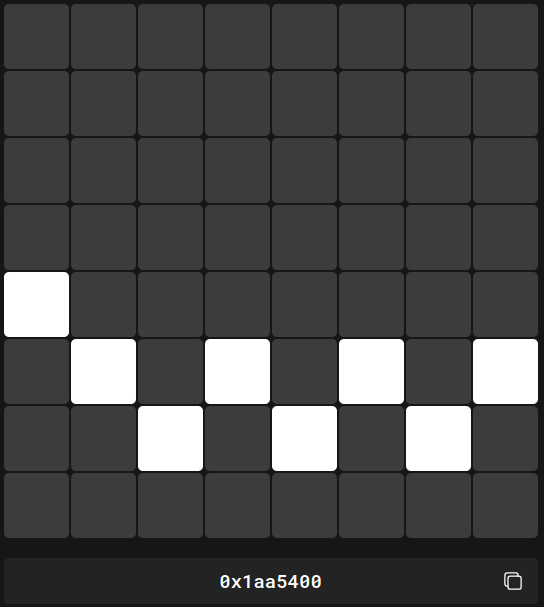
\includegraphics[width=\textwidth]{Imagenes/bitboard_white_pawns.png}
        \caption*{Bitboard of white pawns}
    \end{minipage}
    \hfill
    \begin{minipage}[c]{0.30\textwidth}
        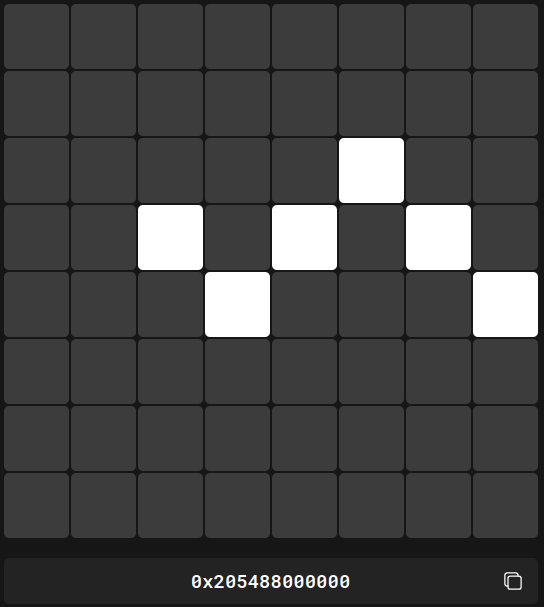
\includegraphics[width=\textwidth]{Imagenes/bitboard_black_pawns.png}
        \caption*{Bitboard of black pawns}
    \end{minipage}
    \hfill
    \begin{minipage}[c]{0.30\textwidth}
        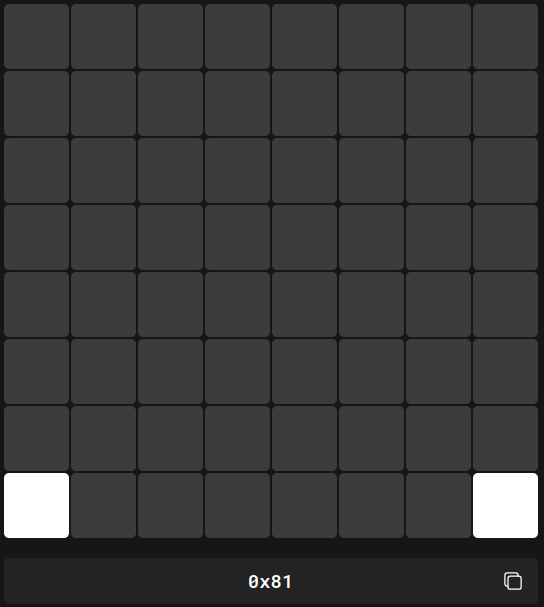
\includegraphics[width=\textwidth]{Imagenes/bitboard_white_rooks.png}
        \caption*{Bitboard of white rooks}
    \end{minipage}
    \caption{List of bitboards data structure example}
    \label{fig:bitboardPositionExample}
    \vspace{-\baselineskip}
\end{figure}

\newpage

\noindent The main advantages of bitboards is that we can operate on multiple squares simultaneously using bitwise operations. For example, we can determine if there are any black pawns on the fifth rank by performing a bitwise AND operation with the corresponding mask. Figure~\ref{fig:bitboardMaskOperation} illustrates this concept.

\begin{figure}[H]
    \centering
    \begin{minipage}[c]{0.30\textwidth}
        \centering
        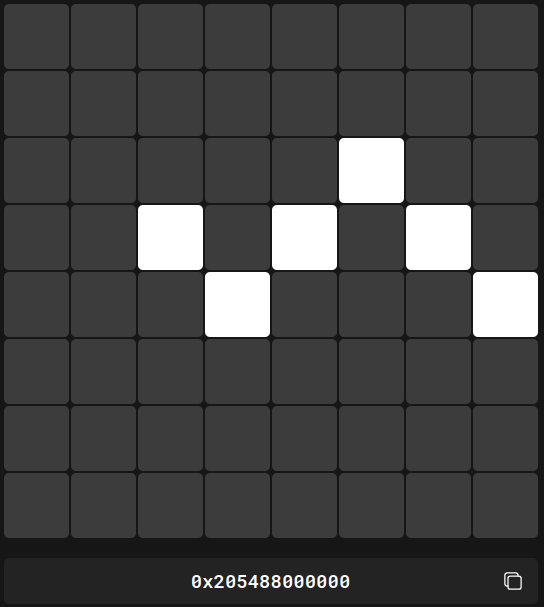
\includegraphics[width=\textwidth]{Imagenes/bitboard_black_pawns.png}
        \caption*{Bitboard of black pawns}
    \end{minipage}
    \hfill
    \begin{minipage}[c]{0.30\textwidth}
        \centering
        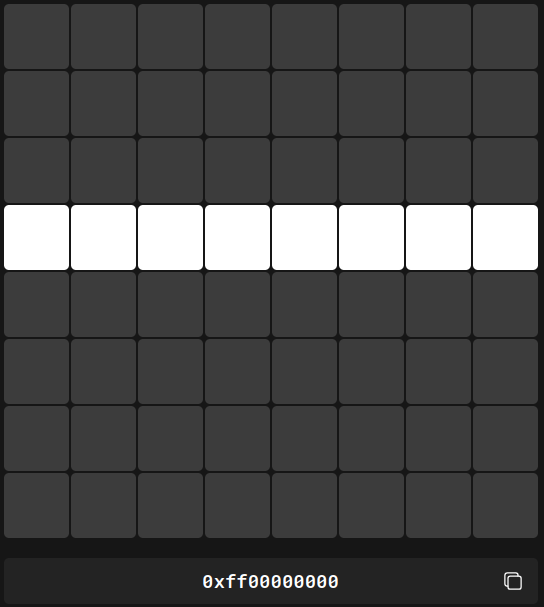
\includegraphics[width=\textwidth]{Imagenes/fifth_rank_mask.png}
        \caption*{Fifth rank mask}
    \end{minipage}
    \hfill
    \begin{minipage}[c]{0.30\textwidth}
        \centering
        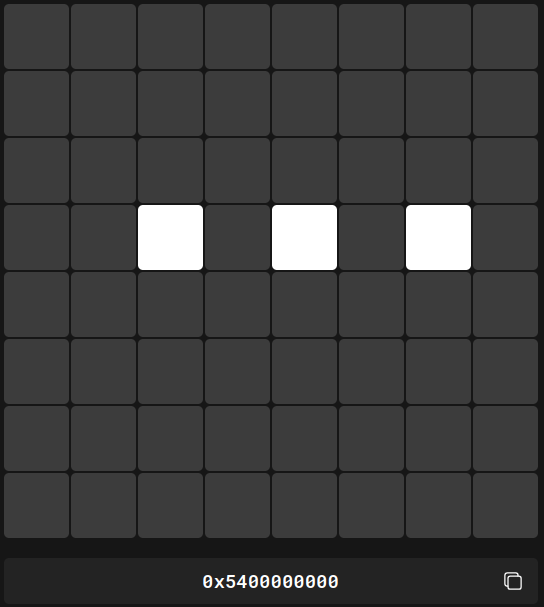
\includegraphics[width=\textwidth]{Imagenes/bitboardMaskResult.png}
        \caption*{Pawn's bitboard \& mask}
    \end{minipage}
    \caption{Bitboard mask operation example}
    \label{fig:bitboardMaskOperation}
\end{figure}

\vspace{2em}

\subsection*{Game State}

\noindent In addition, we need to store the game state information. We designed a compact 64-bit structure to encapsulate all relevant data, enabling efficient copying of the complete game state through a single memory operation. The structure contains the following key fields:

\begin{enumerate}
    \item Total number of moves played in the game [bit 0-19]. 
    \item En passant target square (if applicable) [bits 20-26].
    \item Black's queenside castling availability [bit 27].
    \item Black's kingside castling availability [bit 28].
    \item White's queenside castling availability [bit 29].
    \item White's kingside castling availability [bit 30].
    \item Current side to move (white or black) [bit 31].
    \item Fifty-move rule counter (moves since a capture or pawn move) [bits 35-42].
\end{enumerate}

\vspace{2em}

\noindent Having described the data structures for chess position representation, we now present the engine's core component, the search algorithm.

\newpage

\section{Search Algorithm: The Engine Core}

The search algorithm implemented is minimax enhanced with alpha-beta pruning  where White acts as the maximizing player and Black as the minimizing player. The entire game tree is generated up to a selected maximum depth. At each node, the active player evaluates the position, while the alpha and beta values are dynamically updated during execution. Pruning is performed when a branch of the tree is detected as irrelevant because the evaluation being examined is worse than the current value of alpha (for MAX) or beta (for MIN).

\vspace{1em}

\noindent The complete implementation is available in the basic search file: \\
\scriptsize\url{https://github.com/LauraWangQiu/AlphaDeepChess/blob/main/src/search/search_basic.cpp}\normalsize.

\vspace{2em}

The following events happen at each node of the tree:


\begin{enumerate}
    \item Terminal node verification: Check for game termination conditions including checkmate, threefold repetition, the fifty-move rule, or reaching maximum search depth.
    \item Position evaluation: A positive value indicates White's advantage, while a negative value favors Black. We establish 3,200,000 as the mate-in-one threshold value.
    \item Legal move generation: create a list of every possible legal move in the position.
    \item Move ordering: Sort moves by estimated quality (best to worst). The sooner we explore the best move, the more branches of the tree will be pruned.
    \item Move exploration: Iterate through each of the legal moves from the position in order, update the position evaluation, the value of alpha and beta, and check if we can perform pruning.
\end{enumerate}

\vspace{4em}

\noindent Figure~\ref{fig:alphaBetaExample} demonstrates the alpha-beta search process. The red dashed node is pruned because it cannot influence the final decision independently of its value. If its value is less than or equal to 2, it will never improve the previously analyzed value of 3. On the other hand, if its value is greater than 2, black will still choose 2 to minimize the score. Another formal way to explain this is by using $alpha$ and $beta$ values:

\newpage

\begin{figure}[H]
    \centering
    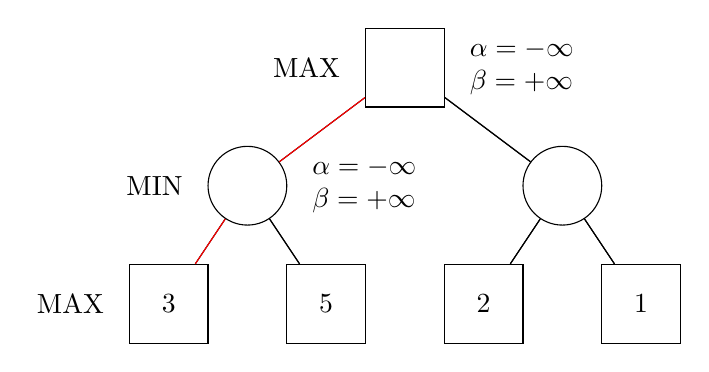
\begin{tikzpicture}[
        level distance=1.5cm,
        level 1/.style={sibling distance=4cm},
        level 2/.style={sibling distance=2cm},
        circleNode/.style={circle, draw, minimum size=1cm, inner sep=0pt},
        squareNode/.style={rectangle, draw, minimum size=1cm, inner sep=0pt}
    ]
        % Root node
        \node[squareNode] (root) {}
            child {node[circleNode] (b) {}
                child {node[squareNode] (d) {3}}
                child {node[squareNode] (e) {5}}
            }
            child {node[circleNode] (c) {}
                child {node[squareNode] (f) {2}}
                child {node[squareNode] (g) {1}}
            };

        % Labels for alpha and beta
        \node[right=0.7cm, align=left] at (root) {$\alpha = -\infty$ \\ $\beta = +\infty$};
        \node[right=0.7cm, align=left] at (b) {$\alpha = -\infty$ \\ $\beta = +\infty$};

        % Node labels
        \node[left=0.7cm] at (root) {MAX};
        \node[left=0.7cm] at (b) {MIN};
        \node[left=0.7cm] at (d) {MAX};

        % Edges
        \draw[-, draw=red] (root) -- (b);
        \draw[-] (root) -- (c);
        \draw[-, draw=red] (b) -- (d);
        \draw[-] (b) -- (e);
        \draw[-] (c) -- (f);
        \draw[-] (c) -- (g);
    \end{tikzpicture}

    \hspace{3em}

    \centering
    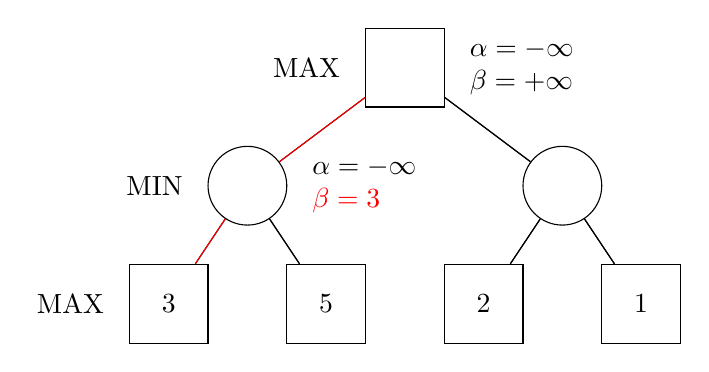
\begin{tikzpicture}[
        level distance=1.5cm,
        level 1/.style={sibling distance=4cm},
        level 2/.style={sibling distance=2cm},
        circleNode/.style={circle, draw, minimum size=1cm, inner sep=0pt},
        squareNode/.style={rectangle, draw, minimum size=1cm, inner sep=0pt}
    ]
        % Root node
        \node[squareNode] (root) {}
            child {node[circleNode] (b) {}
                child {node[squareNode] (d) {3}}
                child {node[squareNode] (e) {5}}
            }
            child {node[circleNode] (c) {}
                child {node[squareNode] (f) {2}}
                child {node[squareNode] (g) {1}}
            };

        % Labels for alpha and beta
        \node[right=0.7cm, align=left] at (root) {$\alpha = -\infty$ \\ $\beta = +\infty$};
        \node[right=0.7cm, align=left] at (b) {$\alpha = -\infty$ \\ $\textcolor{red}{\beta = 3}$};

        % Node labels
        \node[left=0.7cm] at (root) {MAX};
        \node[left=0.7cm] at (b) {MIN};
        \node[left=0.7cm] at (d) {MAX};

        % Edges
        \draw[-, draw=red] (root) -- (b);
        \draw[-] (root) -- (c);
        \draw[-, draw=red] (d) -- (b);
        \draw[-] (b) -- (e);
        \draw[-] (c) -- (f);
        \draw[-] (c) -- (g);
    \end{tikzpicture}

    \hspace{3em}

    \centering
    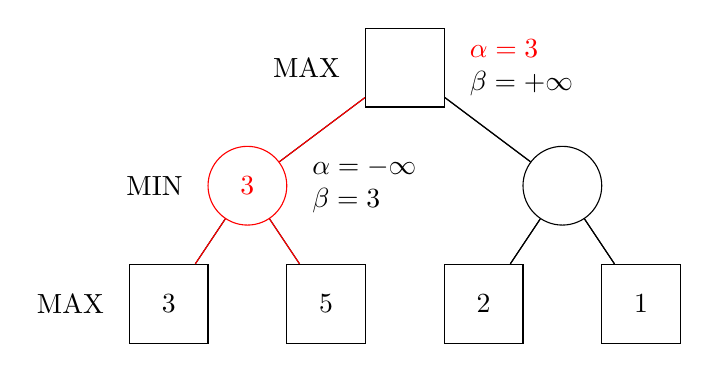
\begin{tikzpicture}[
        level distance=1.5cm,
        level 1/.style={sibling distance=4cm},
        level 2/.style={sibling distance=2cm},
        circleNode/.style={circle, draw, minimum size=1cm, inner sep=0pt},
        squareNode/.style={rectangle, draw, minimum size=1cm, inner sep=0pt}
    ]
        % Root node
        \node[squareNode] (root) {}
            child {node[circleNode, draw=red] (b) {\textcolor{red}{3}}
                child {node[squareNode] (d) {3}}
                child {node[squareNode] (e) {5}}
            }
            child {node[circleNode] (c) {}
                child {node[squareNode] (f) {2}}
                child {node[squareNode] (g) {1}}
            };

        % Labels for alpha and beta
        \node[right=0.7cm, align=left] at (root) {$\textcolor{red}{\alpha = 3}$ \\ $\beta = +\infty$};
        \node[right=0.7cm, align=left] at (b) {$\alpha = -\infty$ \\ $\beta = 3$};

        % Node labels
        \node[left=0.7cm] at (root) {MAX};
        \node[left=0.7cm] at (b) {MIN};
        \node[left=0.7cm] at (d) {MAX};

        % Edges
        \draw[-, draw=red] (root) -- (b);
        \draw[-] (root) -- (c);
        \draw[-, draw=red] (d) -- (b);
        \draw[-, draw=red] (b) -- (e);
        \draw[-] (c) -- (f);
        \draw[-] (c) -- (g);
    \end{tikzpicture}

    \hspace{3em}

    \centering
    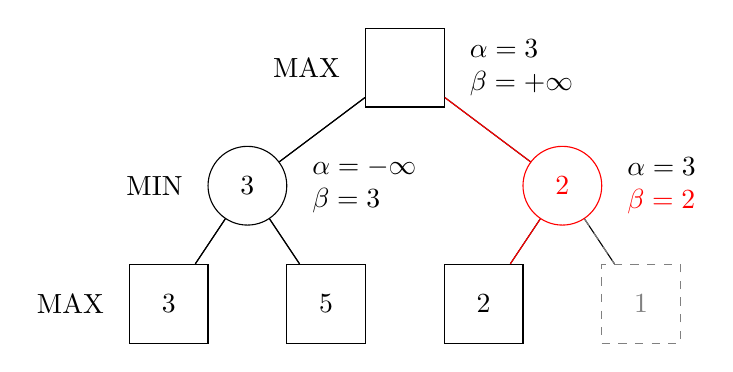
\begin{tikzpicture}[
        level distance=1.5cm,
        level 1/.style={sibling distance=4cm},
        level 2/.style={sibling distance=2cm},
        circleNode/.style={circle, draw, minimum size=1cm, inner sep=0pt},
        squareNode/.style={rectangle, draw, minimum size=1cm, inner sep=0pt}
    ]
        % Root node
        \node[squareNode] (root) {}
            child {node[circleNode] (b) {3}
                child {node[squareNode] (d) {3}}
                child {node[squareNode] (e) {5}}
            }
            child {node[circleNode, draw=red] (c) {\textcolor{red}{2}}
                child {node[squareNode] (f) {2}}
                child {node[squareNode, dashed, gray] (g) {1}}
            };

        % Labels for alpha and beta
        \node[right=0.7cm, align=left] at (root) {$\alpha = 3$ \\ $\beta = +\infty$};
        \node[right=0.7cm, align=left] at (b) {$\alpha = -\infty$ \\ $\beta = 3$};
        \node[right=0.7cm, align=left] at (c) {$\alpha = 3$ \\ $\textcolor{red}{\beta = 2}$};

        % Node labels
        \node[left=0.7cm] at (root) {MAX};
        \node[left=0.7cm] at (b) {MIN};
        \node[left=0.7cm] at (d) {MAX};

        % Edges
        \draw[-] (b) -- (root);
        \draw[-, draw=red] (root) -- (c);
        \draw[-] (d) -- (b);
        \draw[-] (b) -- (e);
        \draw[-, draw=red] (c) -- (f);
        \draw[-, draw=gray, dashed] (c) -- (g);
    \end{tikzpicture}

    \hspace{3em}

    \centering
    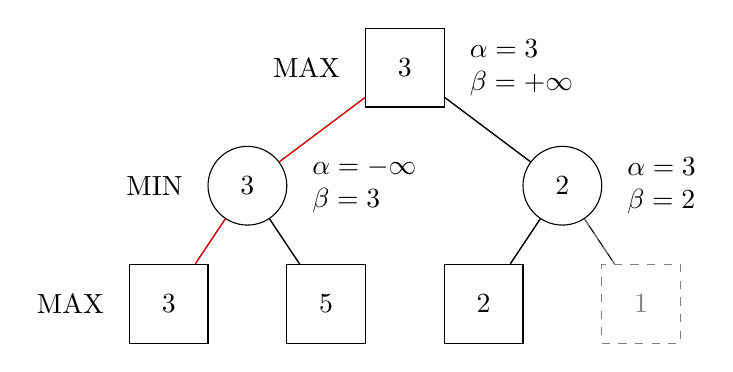
\begin{tikzpicture}[
        level distance=1.5cm,
        level 1/.style={sibling distance=4cm},
        level 2/.style={sibling distance=2cm},
        circleNode/.style={circle, draw, minimum size=1cm, inner sep=0pt},
        squareNode/.style={rectangle, draw, minimum size=1cm, inner sep=0pt}
    ]
        % Root node
        \node[squareNode] (root) {3}
            child {node[circleNode] (b) {3}
                child {node[squareNode] (d) {3}}
                child {node[squareNode] (e) {5}}
            }
            child {node[circleNode] (c) {2}
                child {node[squareNode] (f) {2}}
                child {node[squareNode, dashed, gray] (g) {1}}
            };

        % Labels for alpha and beta
        \node[right=0.7cm, align=left] at (root) {$\alpha = 3$ \\ $\beta = +\infty$};
        \node[right=0.7cm, align=left] at (b) {$\alpha = -\infty$ \\ $\beta = 3$};
        \node[right=0.7cm, align=left] at (c) {$\alpha = 3$ \\ $\beta = 2$};

        % Node labels
        \node[left=0.7cm] at (root) {MAX};
        \node[left=0.7cm] at (b) {MIN};
        \node[left=0.7cm] at (d) {MAX};

        % Edges
        \draw[-, draw=red] (b) -- (root);
        \draw[-] (root) -- (c);
        \draw[-, draw=red] (d) -- (b);
        \draw[-] (b) -- (e);
        \draw[-] (f) -- (c);
        \draw[-, draw=gray, dashed] (c) -- (g);
    \end{tikzpicture}
    \caption{Example of alpha-beta pruning with $\alpha$ and $\beta$ values.}
    \label{fig:alphaBetaExample}
\end{figure}


\subsection*{Iterative deepening}

\noindent What is the optimal depth at which to stop the search? In practice, the most straightforward approach is to perform an iterative deepening search, first searching at depth 1, then 2, then 3\ldots to infinity.~\cite{IterativeDeepening} The engine will update the evaluation and the best move for the position in each iteration. The search can be halted at any point by issuing a \textit{stop} command. In our implementation, this is handled using two threads: one dedicated to reading input from the command line, and the other performing the search. When the stop command is received, the input thread sets an atomic stop flag, which the search thread checks to terminate its execution.

\vspace{1em}

\noindent It is important to note that, in each iteration, all computations from the previous depth are repeated from scratch. This approach is inherently inefficient. In subsequent sections, we will introduce techniques to tackle this inefficiency.

\label{chap:iterativeDeepening}

\subsection*{Horizon effect problem, quiescence search}

What happens if, upon reaching maximum depth, we evaluate the position in the middle of a piece exchange? For example, the figure~\ref{fig:horizonEffectExample} illustrates a position where if the search is stopped when the queen captures the pawn, it will seem like we have won a pawn, but on the next move, another pawn captures the queen, and now we lose a queen. This is known as the horizon effect. ~\cite{HorizonEffect} 

\vspace{1em}

\begin{figure}[H]
    \begin{minipage}{0.4\textwidth}
        \newchessgame
        \chessboard[
            showmover=false,
            setfen=r1bq2kr/pppnppbp/5np1/3p4/3P4/1PNQ1NP1/PBP1PPBP/R5KR w KQkq - 0 1,
            pgfstyle=straightmove, color=blue,
            markmoves={d3-g6},
            arrow=to
        ]
    \end{minipage}
    \hfill
    \begin{minipage}{0.4\textwidth}
        \newchessgame
        \chessboard[
            showmover=false,
            setfen=r1bq2kr/pppnppbp/5nQ1/3p4/3P4/1PN2NP1/PBP1PPBP/R5KR w KQkq - 0 1,
            pgfstyle=straightmove, color=red,
            markmoves={h7-g6},
            arrow=to
        ]
    \end{minipage}

    \caption{Horizon effect position example}
    \label{fig:horizonEffectExample}
\end{figure}

\vspace{1em}

To avoid this, when we reach the end of the tree at maximum depth, we must extend the search but only considering capture moves until no captures are available. This is known as quiescence search. ~\cite{QuiescenceSearch}

\vspace{1em}

\noindent The purpose of this technique is to stop the search only in quiet positions, where there is no capture or tactical movement. Efficiency in this search extension is paramount, as some positions may lead to long sequences of capture moves. To prevent excessive depth, we select a limit of 64 plies, in order to stop the search when we explore to that threshold depth.

\vspace{2em}

The following events occur in a quiescence node:

\vspace{1em}

\begin{enumerate}

    \item Terminal node verification: Check for game termination conditions due to checkmate, threefold repetition, the fifty-move rule or reaching a maximum ply.
    
    \item Standing pat evaluation: Also known as static evaluation, this step assigns a preliminary score to the position. This score can serve as a lower bound and is immediately used to determine whether alpha-beta pruning can be applied.
     
    \item Selective Legal move generation: create a list of every possible legal move excluding moves that are not captures.
    
    \item Move ordering: Sort capture moves by estimated quality (best to worst). The sooner we explore the best move, the more branches of the tree will be pruned.
    
    \item Move exploration: Iterate through each of the capture legal moves from the position in order, update the position evaluation, the value of alpha and beta, and check if we can perform pruning.
    
\end{enumerate}

\subsection*{Aspiration Window}

Aspiration window's main objetive is to reduce the number of nodes to explore by simply restricting the range of alpha and beta values (window). A search is performed with this narrow window. If the position evaluation falls within the window, it is accepted as valid and additional node exploration is avoided. However, if the evaluation is outside the limits of the window (when a fail-low or fail-high occurs), the window is expanded to the extreme values (-INF and +INF) and a new search is performed to obtain an accurate evaluation. ~\cite{AspirationWindow}

\newpage

\section{Evaluation}
\label{sec:evaluation}

In this section we present how our evaluation function works. For each position, a numerical value is assigned representing how favorable the position is for one side: positive (+) for white and negative (-) for black. The values are typically expressed in centipawns (cp), where one centipawn equals one hundredth of a pawn. ~\cite{Shannon1950}

\vspace{1em}

\noindent The full implementation can be found in the following source file: \\
\scriptsize\url{https://github.com/LauraWangQiu/AlphaDeepChess/blob/main/src/evaluation/evaluation_dynamic.cpp}\normalsize.

\vspace{2em}

\noindent Table~\ref{tab:piece-values} shows the standard centipawn values assigned to each piece type:

\begin{table}[H]
    \centering
    \begin{tabular}{|c|c|}
        \hline
        Piece & Value (cp)\\ \hline
        Pawn & 100 \\ \hline
        Knight & 320 \\ \hline
        Bishop & 330 \\ \hline
        Rook & 500 \\ \hline
        Queen & 950 \\ \hline
        King & 500 \\ \hline
    \end{tabular}
    \caption{Standard values assigned to chess pieces in centipawns.}
    \label{tab:piece-values}
\end{table}

\vspace{1em}

\noindent The evaluation of a position can be computed by summing the values of all white pieces on the board and subtracting the values of all black pieces, as shown in the next equation~\ref{fig:materialEvalEquation}.

\begin{figure}[H]
    \centering
    \begin{minipage}{0.8\linewidth}
        \centering
        \begin{equation*}
            \text{Evaluation(position)} = \sum_{w \in \text{WhitePieces}} V(w) - \sum_{b \in \text{BlackPieces}} V(b)
        \end{equation*}
        \vspace{-1em}
    \end{minipage}
    \caption{Materialistic eval formula. Where $V(x)$ denotes the value of piece $x$.}
    \label{fig:materialEvalEquation}
\end{figure}


\vspace{1em}

\subsection*{Piece Square Tables (PST's)}

\noindent The basic material evaluation described earlier has a significant limitatio,  it doesnt consider the fact that a piece could have more power in different squares of the board. For instance, as illustrated in Figure~\ref{fig:knight-movement-corner-and-center}, a knight placed in the center can control up to eight squares, while a knight positioned in the corner can reach only two.

\begin{figure}[H]
    \centering
    \newchessgame
    \chessboard[
        setpieces={Nh8,Nd4},
        showmover=false,
        pgfstyle=straightmove, color=blue,
        markmoves={h8-g6,h8-f7,d4-b5,d4-b3,d4-c2,d4-c6,d4-e6,d4-e2,d4-f5,d4-f3},
        arrow=to
    ]
    \caption{Knight's movement on corner vs in center.}
    \label{fig:knight-movement-corner-and-center}
\end{figure}

\vspace{1em}

\noindent The solution is to add a bonus or a penalization to the piece depending on the square it occupies. This is called a piece square table (PST). For each piece type, a PST assigns a positional bonus based on the square it occupies. These tables are typically implemented as arrays indexed by square and piece type~\cite{PieceSquareTables}.

\vspace{1em}

An example PST for the bishop is shown in Figure~\ref{fig:piece-square-values-bishop}, where the bishop receives a positional bonus for occupying central squares and a penalty for being placed in the edges of the board.

\begin{figure}[H]
    \centering
    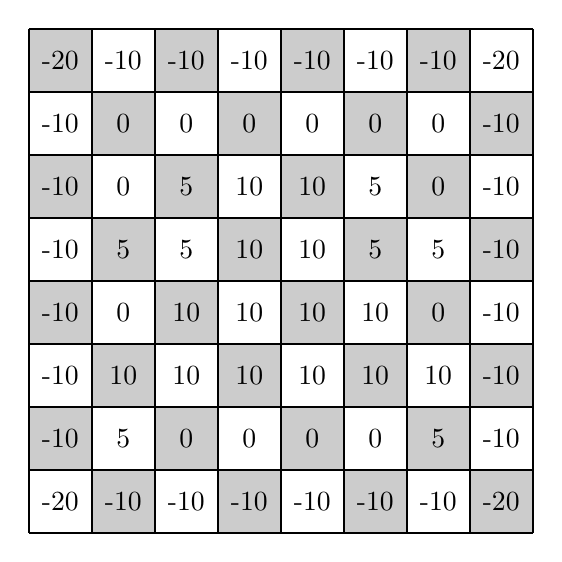
\begin{tikzpicture}[scale=0.8]
        % Draw the chessboard
        \foreach \x in {0,1,...,7} {
            \foreach \y in {0,1,...,7} {
                \pgfmathparse{mod(\x+\y,2) ? "black!20" : "white"}
                \edef\col{\pgfmathresult}
                \fill[\col] (\x,\y) rectangle (\x+1,\y+1);
            }
        }

        % Add the values to the squares
        \node at (0.5,7.5) {-20}; \node at (1.5,7.5) {-10}; \node at (2.5,7.5) {-10}; \node at (3.5,7.5) {-10};
        \node at (4.5,7.5) {-10}; \node at (5.5,7.5) {-10}; \node at (6.5,7.5) {-10}; \node at (7.5,7.5) {-20};

        \node at (0.5,6.5) {-10}; \node at (1.5,6.5) {0}; \node at (2.5,6.5) {0}; \node at (3.5,6.5) {0};
        \node at (4.5,6.5) {0}; \node at (5.5,6.5) {0}; \node at (6.5,6.5) {0}; \node at (7.5,6.5) {-10};

        \node at (0.5,5.5) {-10}; \node at (1.5,5.5) {0}; \node at (2.5,5.5) {5}; \node at (3.5,5.5) {10};
        \node at (4.5,5.5) {10}; \node at (5.5,5.5) {5}; \node at (6.5,5.5) {0}; \node at (7.5,5.5) {-10};

        \node at (0.5,4.5) {-10}; \node at (1.5,4.5) {5}; \node at (2.5,4.5) {5}; \node at (3.5,4.5) {10};
        \node at (4.5,4.5) {10}; \node at (5.5,4.5) {5}; \node at (6.5,4.5) {5}; \node at (7.5,4.5) {-10};

        \node at (0.5,3.5) {-10}; \node at (1.5,3.5) {0}; \node at (2.5,3.5) {10}; \node at (3.5,3.5) {10};
        \node at (4.5,3.5) {10}; \node at (5.5,3.5) {10}; \node at (6.5,3.5) {0}; \node at (7.5,3.5) {-10};

        \node at (0.5,2.5) {-10}; \node at (1.5,2.5) {10}; \node at (2.5,2.5) {10}; \node at (3.5,2.5) {10};
        \node at (4.5,2.5) {10}; \node at (5.5,2.5) {10}; \node at (6.5,2.5) {10}; \node at (7.5,2.5) {-10};

        \node at (0.5,1.5) {-10}; \node at (1.5,1.5) {5}; \node at (2.5,1.5) {0}; \node at (3.5,1.5) {0};
        \node at (4.5,1.5) {0}; \node at (5.5,1.5) {0}; \node at (6.5,1.5) {5}; \node at (7.5,1.5) {-10};

        \node at (0.5,0.5) {-20}; \node at (1.5,0.5) {-10}; \node at (2.5,0.5) {-10}; \node at (3.5,0.5) {-10};
        \node at (4.5,0.5) {-10}; \node at (5.5,0.5) {-10}; \node at (6.5,0.5) {-10}; \node at (7.5,0.5) {-20};

        % Draw the grid
        \draw[thick] (0,0) grid (8,8);
    \end{tikzpicture}
    \caption{Piece Square Table for the bishop.}
    \label{fig:piece-square-values-bishop}
\end{figure}

\subsection*{Tapered evaluation}

\noindent A chess game typically consists of three phases: the opening, where pieces are developed to more effective squares; the middlegame, where tactical and strategic battles take place; and the endgame, where usually the pawns aim to promote and the side that has the advantage tries to corner the enemy king to mate it.

It is clearly suboptimal to assign the same piece-square table (PST) bonuses to pieces like the pawn or king during both the middlegame and the endgame. To address this, we implement \textit{tapered evaluation}, a technique that computes two separate evaluations, one for the middlegame/opening and another for the endgame, then interpolates between the two scores to produce a final evaluation.~\cite{TaperedEvaluation}

\vspace{1em}
\noindent First we calculate the percentage of middlegame and the percentage of endgame:

\begin{enumerate}
    \item 100\% Middlegame: The position includes at least all of the initial minor pieces (2 bishops and 2 knights per side), 2 rooks per side, and both queens.
    \item 100\% Endgame: there are zero minor pieces, zero rooks and zero queens.
\end{enumerate}
\vspace{1em}

\noindent The final tapered evaluation score is computed as a weighted average of the middlegame and endgame evaluations. This is formalized in Equation~\ref{fig:taperedEvalEquation}.

\begin{figure}[H]
    \centering
    \begin{minipage}{0.8\linewidth}
        \centering
        \begin{equation*}
            \text{Eval(position)} = \alpha \cdot \text{middlegameEval} + (1 - \alpha) \cdot \text{endgameEval}
        \end{equation*}
        \vspace{-1em}
    \end{minipage}
    \caption{Tapered evaluation formula, where $\alpha$ represents the proportion of middlegame.}
    \label{fig:taperedEvalEquation}
\end{figure}

\noindent We now need two PST's for each piece, in the following Figure ~\ref{fig:taperedPSTpawns} is the example of the middlegame bonus and the endgame bonus for the pawn, as we can see, the pawns in the endgame receive a bonus for being near the promotion squares.

\begin{figure}[H]
    \begin{minipage}{0.4\textwidth}
        \centering
        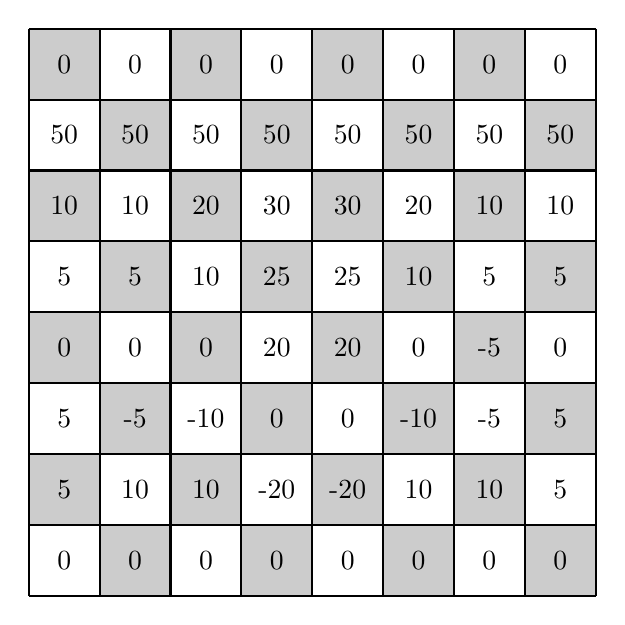
\begin{tikzpicture}[scale=0.9]

            \foreach \x in {0,1,...,7} {
                \foreach \y in {0,1,...,7} {
                    \pgfmathparse{mod(\x+\y,2) ? "black!20" : "white"}
                    \edef\col{\pgfmathresult}
                    \fill[\col] (\x,\y) rectangle (\x+1,\y+1);
                }
            }

            \node at (0.5,7.5) {0};   \node at (1.5,7.5) {0};   \node at (2.5,7.5) {0};   \node at (3.5,7.5) {0};
            \node at (4.5,7.5) {0};   \node at (5.5,7.5) {0};   \node at (6.5,7.5) {0};   \node at (7.5,7.5) {0};

            \node at (0.5,6.5) {50};  \node at (1.5,6.5) {50};  \node at (2.5,6.5) {50};  \node at (3.5,6.5) {50};
            \node at (4.5,6.5) {50};  \node at (5.5,6.5) {50};  \node at (6.5,6.5) {50};  \node at (7.5,6.5) {50};

            \node at (0.5,5.5) {10};  \node at (1.5,5.5) {10};  \node at (2.5,5.5) {20};  \node at (3.5,5.5) {30};
            \node at (4.5,5.5) {30};  \node at (5.5,5.5) {20};  \node at (6.5,5.5) {10};  \node at (7.5,5.5) {10};

            \node at (0.5,4.5) {5};   \node at (1.5,4.5) {5};   \node at (2.5,4.5) {10};  \node at (3.5,4.5) {25};
            \node at (4.5,4.5) {25};  \node at (5.5,4.5) {10};  \node at (6.5,4.5) {5};   \node at (7.5,4.5) {5};

            \node at (0.5,3.5) {0};   \node at (1.5,3.5) {0};   \node at (2.5,3.5) {0};   \node at (3.5,3.5) {20};
            \node at (4.5,3.5) {20};  \node at (5.5,3.5) {0};   \node at (6.5,3.5) {-5};  \node at (7.5,3.5) {0};

            \node at (0.5,2.5) {5};   \node at (1.5,2.5) {-5};  \node at (2.5,2.5) {-10}; \node at (3.5,2.5) {0};
            \node at (4.5,2.5) {0};   \node at (5.5,2.5) {-10}; \node at (6.5,2.5) {-5};  \node at (7.5,2.5) {5};
            
            \node at (0.5,1.5) {5};   \node at (1.5,1.5) {10};  \node at (2.5,1.5) {10};  \node at (3.5,1.5) {-20};
            \node at (4.5,1.5) {-20}; \node at (5.5,1.5) {10};  \node at (6.5,1.5) {10};  \node at (7.5,1.5) {5};

            \node at (0.5,0.5) {0};   \node at (1.5,0.5) {0};   \node at (2.5,0.5) {0};   \node at (3.5,0.5) {0};
            \node at (4.5,0.5) {0};   \node at (5.5,0.5) {0};   \node at (6.5,0.5) {0};   \node at (7.5,0.5) {0};

            \draw[thick] (0,0) grid (8,8);
        \end{tikzpicture}
        \caption*{Pawn middlegame PST}
    \end{minipage}
    \hfill
    \begin{minipage}{0.4\textwidth}
        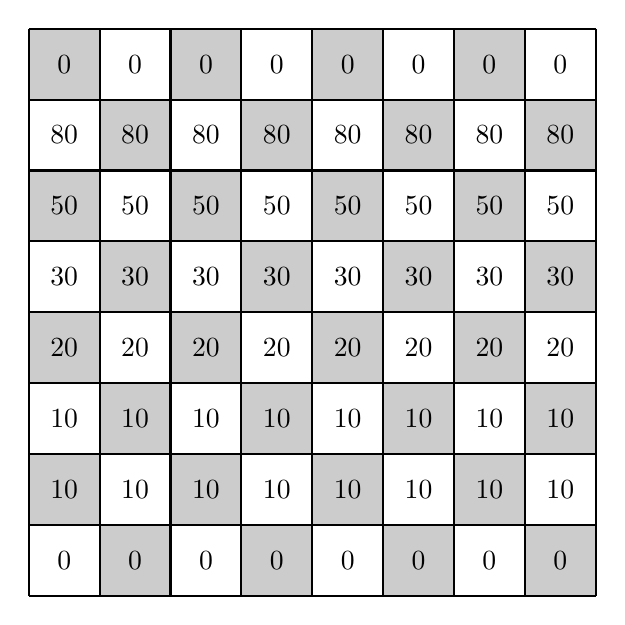
\begin{tikzpicture}[scale=0.9]

            \foreach \x in {0,1,...,7} {
                \foreach \y in {0,1,...,7} {
                    \pgfmathparse{mod(\x+\y,2) ? "black!20" : "white"}
                    \edef\col{\pgfmathresult}
                    \fill[\col] (\x,\y) rectangle (\x+1,\y+1);
                }
            }

            \node at (0.5,7.5) {0}; \node at (1.5,7.5) {0}; \node at (2.5,7.5) {0}; \node at (3.5,7.5) {0};
            \node at (4.5,7.5) {0}; \node at (5.5,7.5) {0}; \node at (6.5,7.5) {0}; \node at (7.5,7.5) {0};

            \node at (0.5,6.5) {80}; \node at (1.5,6.5) {80}; \node at (2.5,6.5) {80}; \node at (3.5,6.5) {80};
            \node at (4.5,6.5) {80}; \node at (5.5,6.5) {80}; \node at (6.5,6.5) {80}; \node at (7.5,6.5) {80};

            \node at (0.5,5.5) {50}; \node at (1.5,5.5) {50}; \node at (2.5,5.5) {50}; \node at (3.5,5.5) {50};
            \node at (4.5,5.5) {50}; \node at (5.5,5.5) {50}; \node at (6.5,5.5) {50}; \node at (7.5,5.5) {50};

            \node at (0.5,4.5) {30}; \node at (1.5,4.5) {30}; \node at (2.5,4.5) {30}; \node at (3.5,4.5) {30};
            \node at (4.5,4.5) {30}; \node at (5.5,4.5) {30}; \node at (6.5,4.5) {30}; \node at (7.5,4.5) {30};

            \node at (0.5,3.5) {20}; \node at (1.5,3.5) {20}; \node at (2.5,3.5) {20}; \node at (3.5,3.5) {20};
            \node at (4.5,3.5) {20}; \node at (5.5,3.5) {20}; \node at (6.5,3.5) {20}; \node at (7.5,3.5) {20};

            \node at (0.5,2.5) {10}; \node at (1.5,2.5) {10}; \node at (2.5,2.5) {10}; \node at (3.5,2.5) {10};
            \node at (4.5,2.5) {10}; \node at (5.5,2.5) {10}; \node at (6.5,2.5) {10}; \node at (7.5,2.5) {10};

            \node at (0.5,1.5) {10}; \node at (1.5,1.5) {10}; \node at (2.5,1.5) {10}; \node at (3.5,1.5) {10};
            \node at (4.5,1.5) {10}; \node at (5.5,1.5) {10}; \node at (6.5,1.5) {10}; \node at (7.5,1.5) {10};

            \node at (0.5,0.5) {0}; \node at (1.5,0.5) {0}; \node at (2.5,0.5) {0}; \node at (3.5,0.5) {0};
            \node at (4.5,0.5) {0}; \node at (5.5,0.5) {0}; \node at (6.5,0.5) {0}; \node at (7.5,0.5) {0};

            \draw[thick] (0,0) grid (8,8);
        \end{tikzpicture}
        \caption*{Pawn endgame PST}
    \end{minipage}
    \caption{Tapered Piece Square Tables for pawn.}
    \label{fig:taperedPSTpawns}
\end{figure}

\newpage

\section{Move Ordering}

\noindent Having explained the evaluation function, in this chapter we detail the implementation of the move ordering heuristic.

\vspace{1em}

\noindent The complete implementation can be found in the following file:\\
\scriptsize\url{https://github.com/LauraWangQiu/AlphaDeepChess/blob/main/src/move_ordering/move_ordering_MVV_LVA.cpp}\normalsize.

\vspace{1em}

\noindent During the search process, the earlier we explore the best move in a position, the better the algorithm performs. In the best-case scenario, if the first move explored is indeed the optimal one, the remaining branches of the tree can be pruned. To achieve this, we sort the legal moves by estimated quality, from best to worst~\cite{MoveOrdering}.

\subsection*{Most Valuable Victim - Least Valuable Aggressor (MVV-LVA)}

\noindent The heuristic we implemented is the Most Valuable Victim - Least Valuable Aggressor (MVV-LVA). In this approach, a move receives a high score if it captures a valuable piece using a less valuable one. For example, capturing a queen with a pawn is considered a very strong move~\cite{MVVLVA}.

\vspace{1em}

\noindent We implemented this heuristic using a look-up table indexed by the moving piece and the captured piece, as shown in Table~\ref{tab:mvv-lva-table}. Capturing a queen with a pawn receives a score of 55, while doing the opposite receives 11 points.

\begin{table}[H]
    \centering
    \begin{tabular}{|c|c|c|c|c|c|c|c|}
    \hline
    \textit{Victim $\backslash$ Attacker} & \textit{P} & \textit{N} & \textit{B} & \textit{R} & \textit{Q} & \textit{K} & \textit{EMPTY} \\
    \hline
    \textit{P}     & 15 & 14 & 13 & 12 & 11 & 10 & 0 \\
    \textit{N}     & 25 & 24 & 23 & 22 & 21 & 20 & 0 \\
    \textit{B}     & 35 & 34 & 33 & 32 & 31 & 30 & 0 \\
    \textit{R}     & 45 & 44 & 43 & 42 & 41 & 40 & 0 \\
    \textit{Q}     & 55 & 54 & 53 & 52 & 51 & 50 & 0 \\
    \textit{K}     &  0 &  0 &  0 &  0 &  0 &  0 & 0 \\
    \textit{EMPTY} &  0 &  0 &  0 &  0 &  0 &  0 & 0 \\
    \hline
    \end{tabular}
    \caption{MVV-LVA heuristic table: Rows = Victims, Columns = Attackers.}
    \label{tab:mvv-lva-table}
\end{table}

\subsection*{Killer moves}

The main limitation of MVV-LVA is that it only applies to capture moves. In fact, assigning meaningful scores to non-capturing (quiet) moves is a challenging task. To address this, we implemented the \textit{killer move} heuristic, which assigns high scores to certain quiet moves.

\vspace{1em}

A \textit{killer move} is a quiet, non-capturing move which can cause a cutoff in different branches of the tree at the same depth.~\cite{KillerMoves}

\vspace{1em}

Figure~\ref{fig:killer_move_example} shows an example of a killer move.

\begin{figure}[H]
    \centering
    \begin{minipage}{0.6\textwidth}
        \centering
        \newchessgame
        \chessboard[
            showmover=false,
            setfen=1r3k2/ppp2ppp/1n1bp3/q2p2N1/3P4/2P1P3/PP3PPP/2BQ2KR w K - 0 3,
            pgfstyle=straightmove, color=blue,
            markmoves={d1-h5},
            arrow=to,
            markstyle=circle,
            color=red, markfields={f7}
        ]
    \end{minipage}

    \caption{Killer move example. The queen moves to h5, threatening checkmate on f7. This prunes all other moves that do not respond to the threat.}
    \label{fig:killer_move_example}
\end{figure}

\vspace{1em}

\noindent These moves are remembered and prioritized during move ordering, as they have proven effective in position at the same depth in the search tree. We implemented a table where we store two moves that causes a cutoff per search depth. There could be more than two killer moves, our replacement policy is to always mantain the older killer move found in one slot, and in the other slot store the least recently found.

\vspace{1em}

\noindent If a quiet move being evaluated matches one of the killer moves stored at the current search depth, we increase its score by 70 points.

\newpage

\section{Improvements}

\noindent Some improvements and new structures were later added for different versions: transposition tables, Zobrist hashing, table entries, PEXT instructions, search multithread and search reductions that will be discussed and analysed below.

\vspace{1em}

\noindent At the end of each section, we present the results of the 100-game match between the engine with the implemented technique and a baseline version, which includes only the fundamental techniques described in the previous chapters. The objective of these tests are to evaluate the difference in playing strength introduced by the new implementation.

\subsection{Transposition Table}
\label{sec:tt}

\noindent As discused in the previous chapter (see Section~\ref{chap:iterativeDeepening}), the basic implementation of the chess engine generates a large amount of redundant calculations due to the iterative deepening approach and also the concept of transpositions: situations in which the same board position is reached through different sequences of moves in the game tree.
\noindent Figure~\ref{fig:transposition_example} illustrates a position that can arise through multiple move orders. Where the white king could go to the g3 square from multiple paths.

\begin{figure}[H]
    \centering
    \begin{minipage}{0.6\textwidth}
        \centering
        \newchessgame
        \chessboard[
            showmover=false,
            setfen=8/2k5/3p4/p2P1p2/P2P1P2/8/8/2K5 w - - 0 1,
            pgfstyle=straightmove, color=blue,
            markmoves={c1-e3,e3-g3,c1-g1,g1-g3},
            arrow=to
        ]
    \end{minipage}
    \caption{Lasker-Reichhelm Position, transposition example}
    \label{fig:transposition_example}
\end{figure}

\vspace{1em}

\noindent Taking advantage of the concept of dynamic programming, we create a look-up table of chess positions and its evaluation. So if we encounter the same position again, the evaluation is already precalculated. However, we ask ourselves the following question: how much space does the look-up table take up if there are an astronomical amount of chess positions? What we can do is assign a hash to each position and make the table index the last bits of the hash. The larger the table, the less likely access collisions will be. We also want a hash that is fast to calculate and has collision-reducing properties; for this, we will use the Zobrist hashing technique in the following subsection.

\vspace{1em}

\subsubsection{Zobrist Hashing}

Zobrist Hashing is a technique to transform a board position of arbitrary size into a number of a set length, with an equal distribution over all possible numbers invented by Albert Zobrist. (\cite{ZobristHashing})

\vspace{1em}

\noindent To generate a 64-bit hash for a position, the following steps are followed:

\begin{itemize}
  \item There are 12 different types of chess pieces. For each of the 64 squares on the board, we generate 12 random 64-bit integers. That is, each piece-square combination is assigned a unique random value. This initialization step is performed only once when the program starts.
  \item The hash value for a given position is computed by performing the XOR operation between the hash accumulator and the random value corresponding to each piece on its square.
  \item In addition to the pieces, we also include:
  \begin{itemize}
    \item A random value for the side to move.
    \item One random value to account for the possibility of an en passant capture.
    \item One random value per possible castling move.
  \end{itemize}
  \item These random values are useful so that even slightly different positions produce very different hash values. This greatly reduces the chance of collisions.
  \item The XOR operation is used not only because it is computationally inexpensive, but also because it is reversible. This means that when a move is made or undone, we can update the hash incrementally by applying XOR only to the affected squares, without needing to recompute the entire hash.
\end{itemize}

\begin{lstlisting}[breaklines=true, frame=single, caption={Code example to calculate zobrist hash of position}, label={lst:zobrist_calculate_hash}]
/**
 * @brief Calculate zobrist hash of position
 * 
 * @param[in] position board containing the chess position
 * 
 * @return the hash key of the chess position
 * 
 */
static uint64_t hash(const Board& position)
{
    // initialize the random numbers only once
    init_random_numbers_only_once();   

    uint64_t hash = 0ULL;

    for (Square square = Square::A1; square.is_valid(); square++) {
        const Piece piece = position.get_piece(square);
        if (piece != Piece::EMPTY) {
            hash ^= get_seed(square, piece);
        }
    }
    const GameState state = position.state();

    const Square eps_square = state.en_passant_square();
    if (eps_square.is_valid()) {
        hash ^= get_en_passant_seed(eps_square.col());
    }

    if (state.castle_king_white()) {
        hash ^= get_king_white_castle_seed();
    }
    if (state.castle_queen_white()) {
        hash ^= get_queen_white_castle_seed();
    }
    if (state.castle_king_black()) {
        hash ^= get_king_black_castle_seed();
    }
    if (state.castle_queen_black()) {
        hash ^= get_queen_black_castle_seed();
    }

    if (state.side_to_move() == ChessColor::BLACK) {
        hash ^= get_black_to_move_seed();
    }

    return hash;
}
\end{lstlisting}

\subsubsection{Table Entry}

Each entry in the transposition table stores the following information:

\begin{itemize}
  \item Zobrist Hash: The full 64-bit hash of the position. This is used to verify that the entry corresponds to the current position and to detect possible index collisions in the table.
  \item Evaluation: The numerical evaluation of the position, as computed by the evaluation function.
  \item Depth: The depth at which the evaluation was calculated. A deeper search could potentially yield a more accurate evaluation, so this value helps determine whether a new evaluation should overwrite the existing one.
  \item Node Type: Indicates the type of node stored:
  \begin{itemize}
    \item \texttt{EXACT} the evaluation is precise for this position.
    \item \texttt{UPPERBOUND} the evaluation is an upper bound, typically resulting from an alpha cutoff.
    \item \texttt{LOWERBOUND} the evaluation is a lower bound, typically resulting from a beta cutoff.
    \item \texttt{FAILED} entry is empty or with invalid information.
  \end{itemize}
\end{itemize}

\begin{lstlisting}[breaklines=true, frame=single, caption={Code example transposition table entry}, label={lst:transposition_table_entry}]
class TranspositionTable::Entry
{
    uint64_t key; // full Zobrist key of the chess position

    int evaluation; // Score of the chess position

    Move move; // Best move found for the position.

    NodeType type; // FAILED, EXACT, LOWERBOUND, UPPERBOUND

    int8_t depth; // At which the position was evaluated
...
}
\end{lstlisting}

\subsubsection{Collisions}

As discussed earlier, index collisions in the transposition table are handled by verifying the full Zobrist hash stored in the entry. However, it is still theoretically possible for a full hash collision to occur, that is two different positions producing the same hash.

\vspace{1em}

\noindent This scenario is extremely rare. With 64-bit hashes, there are $2^{64}$ possible unique values, which is more than sufficient for practical purposes. In the unlikely event of a true hash collision, it could result in an incorrect evaluation being reused for a different position.

\subsubsection{Analysis}

To evaluate the improvement introduced by the transposition table, we conducted a 100-game tournament against the basic version of the engine. We selected 50 random starting positions from an opening book and played each position twice, alternating colors to ensure fairness. Each bot has 4 seconds to think per move.

\begin{center}
\begin{figure}[H]
    \centering
    \ResultBar{15cm}{0.5cm}{46}{22}{32}
    \caption{64MB Transposition Table bot vs basic bot}
    \label{fig:results_transposition_table_bot}
\end{figure}
\medskip
\end{center}

\noindent We see a substantial improvement by adding the transposition table with 46 wins versus 32 losses.

\subsection{Move generator with Magic Bitboards and PEXT instructions}

To identify potential performance bottlenecks, we performed profiling on the engine.

\begin{center}
    \begin{figure}[H]
    \centering
        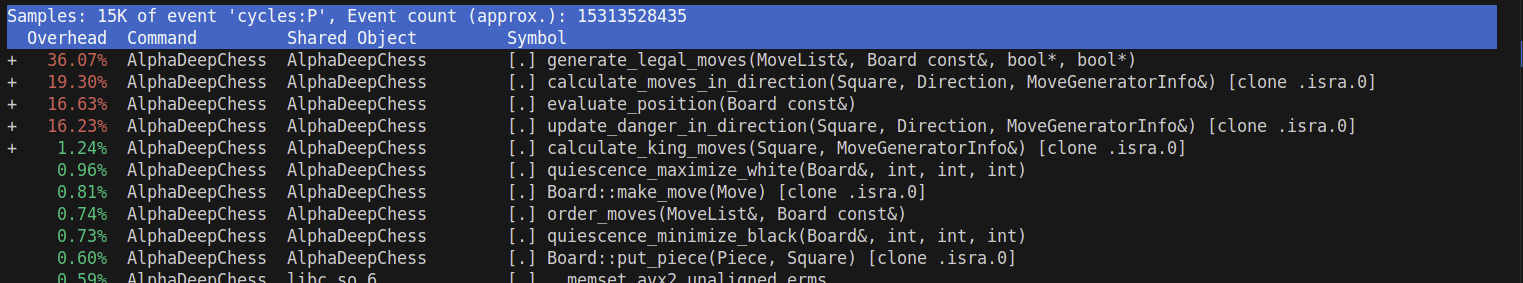
\includegraphics[width=1.0\textwidth]{Imagenes/basic_move_generator_profiling.png}
        \caption{Profiling results}
        \label{fig:profiling}
    \end{figure}
    \medskip
\end{center}


\noindent Profiling results show that most part of the total execution time is spent in the generate legal moves function. Therefore, optimizing this component is expected to lead to significant performance improvements.

\subsubsection{Magic bitboards}

We can create a look up table of all the rook and bishop moves for each square on the board and for each combination of pieces that blocks the path of the slider piece (blockers  bitboard). Basically we need a hash table to store rook and bishop moves indexed by square and bitboard of blockers. The problem is that this table could be very big.~\cite{MagicBitboards}

\vspace{1em}

\noindent Magic bitboards technique used to reduce the size of the look up table. We cut off unnecesary information in the blockers bitboard, excluding the board borders and the squares outside its attack pattern.

\vspace{1em}

A \textbf{magic number} is a multiplier to the bitboard of blockers with the following properties:

\begin{itemize}
  \item Preserves relevant blocker information: 
  The nearest blockers along a piece's movement direction are preserved. 
  \textit{Example:} Consider a rook with two pawns in its path:
  \begin{lstlisting}[breaklines=true]
    Rook -> -> -> [Pawn1][Pawn2]
  \end{lstlisting}
  In this case, only `Pawn1` blocks the rook's movement, while `Pawn2` is irrelevant.
  \item Compresses the blocker bitboard, pushing the important bits near the most significant bit.
  \item The final multiplication must produce a unique index for each possible blocker configuration. The way to ensure the uniqueness is by brute force testing.
\end{itemize}

\noindent As illustrated in Figure~\ref{fig:magics_position}, we aim to compute the legal moves of the white rook in the given position. In practice, the only pieces that truly block the rook's path are those marked with a red circle.

\begin{figure}[H]
    \centering
    \begin{minipage}{0.6\textwidth}
        \centering
        \newchessgame
        \chessboard[
            showmover=false,
            setfen=n1bk3r/3p4/1p1p2p1/8/3R1p2/8/3p4/7n w - - 0 1,
            markstyle=circle,
            color=red, markfields={d6,f4,d2},
            color=green, markfields={c4,b4,a4,e4,d5,d3}
        ]
    \end{minipage}
    \caption{Initial chess position with white rook and blockers}
    \label{fig:magics_position}
\end{figure}

\noindent First, we mask out all pieces outside the rook's attack pattern or on the board borders, as shown in Figure~\ref{fig:magic_preprocessing}.

\begin{figure}[H]
    \centering
    \begin{minipage}[c]{0.4\textwidth}
        \centering
        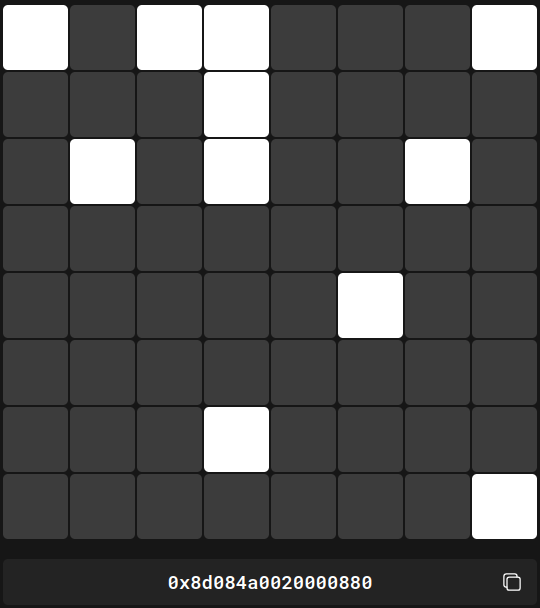
\includegraphics[width=\textwidth]{Imagenes/magics_blockers.png}
        \caption*{Original blockers bitboard}
    \end{minipage}
    \hfill
    \begin{minipage}[c]{0.1\textwidth}
        \centering
        \small$\to$
    \end{minipage}
    \hfill
    \begin{minipage}[c]{0.4\textwidth}
        \centering
        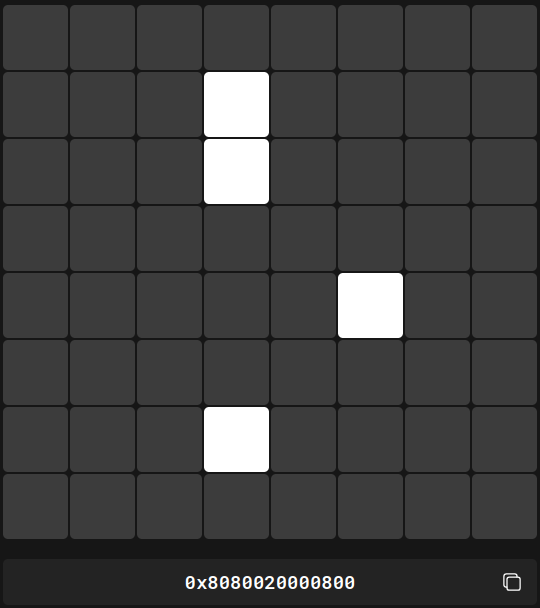
\includegraphics[width=\textwidth]{Imagenes/magics_processed_blockers.png}
        \caption*{Masked blockers bitboard}
    \end{minipage}
    \caption{Pre-processing of the blockers bitboard}
    \label{fig:magic_preprocessing}
\end{figure}

\noindent As illustrated in Figure~\ref{fig:magic_multiplication}, the masked blockers bitboard is then multiplied by the magic number. The result retains only the three relevant pawns that obstruct the rook's movement, pushing them toward the most significant bits.

\begin{figure}[H]
    \centering
    \begin{minipage}[c]{0.4\textwidth}
        \centering
        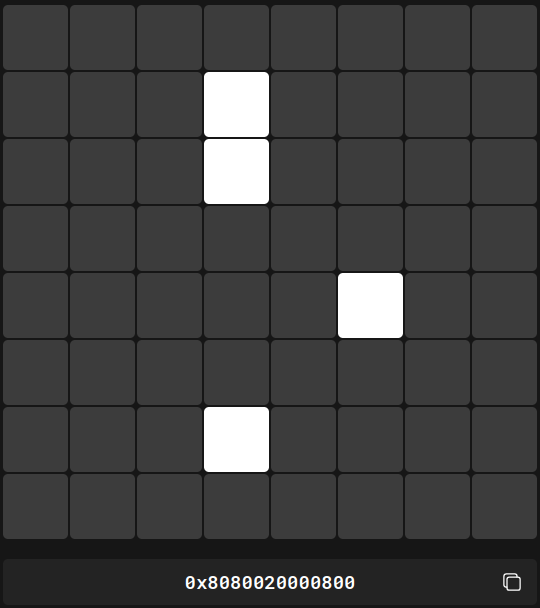
\includegraphics[width=\textwidth]{Imagenes/magics_processed_blockers.png}
        \caption*{Masked blockers bitboard}
    \end{minipage}
    \hfill
    \begin{minipage}[c]{0.1\textwidth}
        \centering
        \Huge$\times$ \\[0.5em]
        \small Magic number \\[0.5em]
        \Huge$=$
    \end{minipage}
    \hfill
    \begin{minipage}[c]{0.4\textwidth}
        \centering
        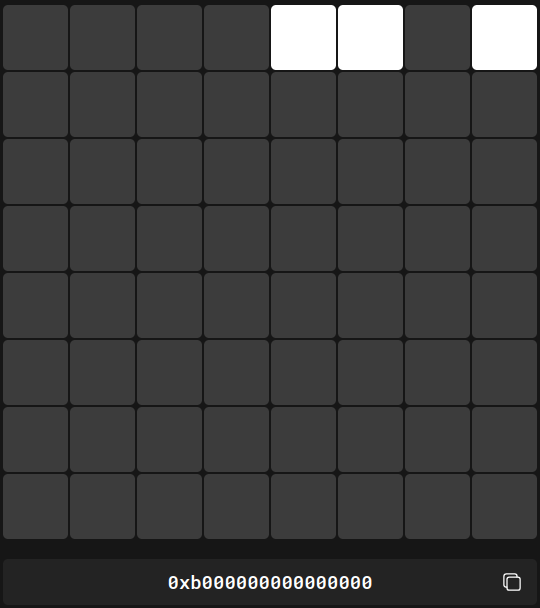
\includegraphics[width=\textwidth]{Imagenes/magics_multiplied_blockers.png}
        \caption*{Multiplied blockers bitboard}
    \end{minipage}
    \caption{Multiplication by magic number to produce an index}
    \label{fig:magic_multiplication}
\end{figure}

\noindent Next, we compress the index toward the least significant bits by shifting right by \(\,64-\)\texttt{relevant\_squares}. The number of relevant squares varies per board square; Listing~\ref{lst:rook_relevant_squares} shows this for the rook:

\begin{lstlisting}[breaklines=true, frame=single, caption={Number of relevant squares for each rook square}, label={lst:rook_relevant_squares}]
/**
 * @brief ROOK_RELEVANT_SQUARES
 * 
 * Number of squares where the rook could move
 * from each square minus the board border squares.
 */
static constexpr int ROOK_RELEVANT_SQUARES[NUM_SQUARES] =
{
    12, 11, 11, 11, 11, 11, 11, 12,
    11, 10, 10, 10, 10, 10, 10, 11,
    11, 10, 10, 10, 10, 10, 10, 11,
    11, 10, 10, 10, 10, 10, 10, 11,
    11, 10, 10, 10, 10, 10, 10, 11,
    11, 10, 10, 10, 10, 10, 10, 11,
    11, 10, 10, 10, 10, 10, 10, 11,
    12, 11, 11, 11, 11, 11, 11, 12
};
\end{lstlisting}

\vspace{1em}

\noindent The final index is thus computed as:

\begin{align*}
    \text{index}
    &= (\texttt{bitboard\_of\_blockers} \times \texttt{magic\_number})
       \;\gg\;(64 - \texttt{relevant\_squares})\,.
\end{align*}

\subsubsection{PEXT instruction}

\noindent The \texttt{PEXT} (Parallel Bits Extract) instruction—available on modern x86\_64 CPUs—extracts bits from a source operand according to a mask and packs them into the lower bits of the destination operand.~\cite{PextInstruction} It is ideally suited for computing our table index.

Figure~\ref{fig:pext_instruction_example} illustrates how \texttt{PEXT} works: it selects specific bits from register \texttt{r2}, as specified by the mask in \texttt{r3}, and packs the result into the lower bits of the destination register \texttt{r1}.

\begin{figure}[H]
    \centering
    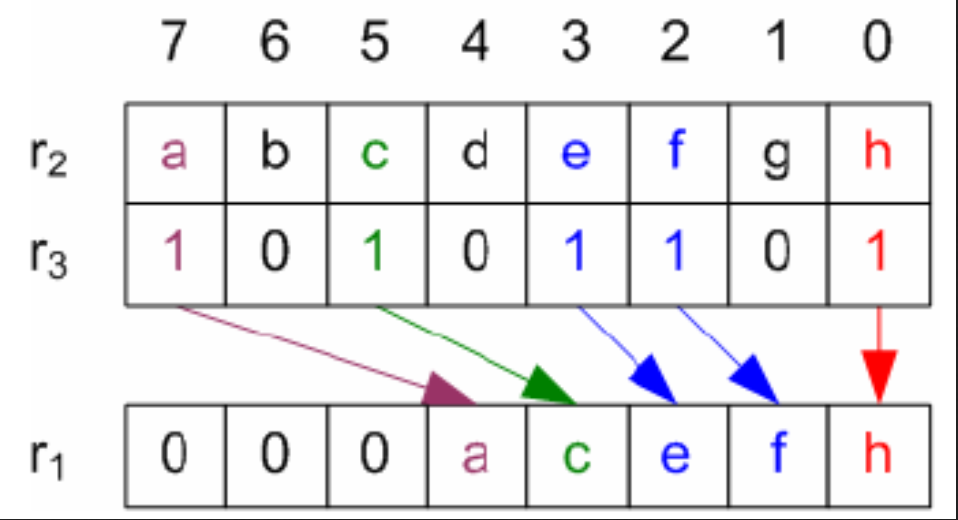
\includegraphics[width=0.5\textwidth]{Imagenes/pext.png}
    \caption{Example of the \texttt{PEXT} instruction: extracting bits from \texttt{r2} using \texttt{r3} as a mask, and storing the result in \texttt{r1}. ~\cite{PextInstruction}}
    \label{fig:pext_instruction_example}
\end{figure}

\noindent For our previous example (see Figure~\ref{fig:magics_position}), we only need the full bitboard of blockers and the rook’s attack pattern (excluding the borders to reduce space), as illustrated in Figure~\ref{fig:pext_bitboards}.

\begin{figure}[H]
    \centering
    \begin{minipage}[c]{0.3\textwidth}
        \centering
        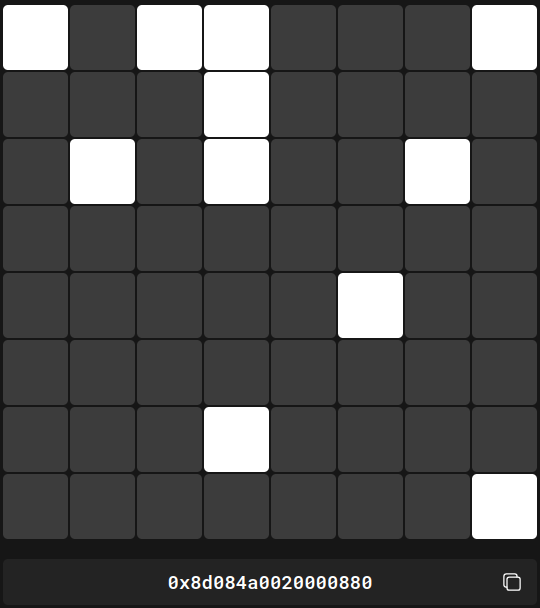
\includegraphics[width=\textwidth]{Imagenes/magics_blockers.png}
        \caption*{Blockers bitboard}
    \end{minipage}
    \hfill
    \begin{minipage}[c]{0.3\textwidth}
        \centering
        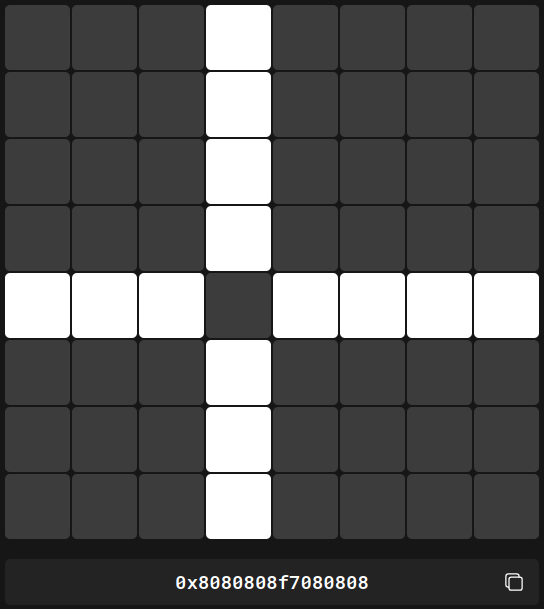
\includegraphics[width=\textwidth]{Imagenes/magics_rook_attacks.png}
        \caption*{Rook attack mask}
    \end{minipage}
    \hfill
    \begin{minipage}[c]{0.05\textwidth}
        \centering
        \Huge\texttt{->}
    \end{minipage}
    \hfill
    \begin{minipage}[c]{0.3\textwidth}
        \centering
        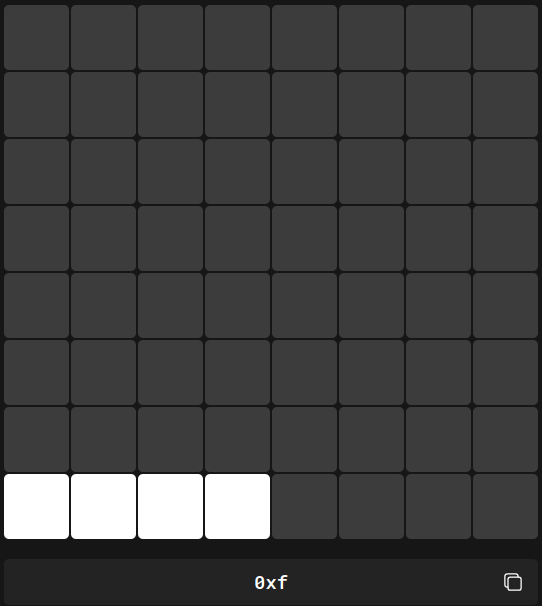
\includegraphics[width=\textwidth]{Imagenes/pext_final_index.png}
        \caption*{Final extracted index}
    \end{minipage}
    \caption{index extraction with Pext example}
    \label{fig:pext_bitboards}
\end{figure}

\noindent The final index used to access the lookup table is calculated using the \texttt{pext} instruction as follows:

\begin{align*}
    \text{index}
    &= \texttt{\_pext\_u64}(\texttt{blockers},\,\texttt{attack\_pattern})\,.
\end{align*}

\noindent To maintain compatibility and performance across different hardware platforms, we provide two implementations:

\begin{itemize}
  \item If \texttt{PEXT} support is detected at compile time, the engine uses it to compute the index directly.
  \item Otherwise, the engine falls back to the Magic Bitboards approach using multiplication and bit shifts.
\end{itemize}

\subsubsection{Analysis}

To evaluate the improvement in the move generator, we conducted the same 
100 game match vs the basic bot version.

\begin{center}
    \begin{figure}[H]
        \centering
        \ResultBar{15cm}{0.5cm}{64}{14}{22}
        \caption{Move generator with PEXT instructions bot vs basic bot}
        \label{fig:results_pext_move_generator_bot}
    \end{figure}
\medskip
\end{center}

\noindent Huge improvement with 64 wins versus 22 losses.

\subsection{Evaluation with King Safety and piece mobility}

It is often beneficial to evaluate additional aspects of a position beyond simply counting material. We introduce the following positional evaluation parameters:

\begin{enumerate}
    \item King Shield Bonus: The king is typically safer when protected by friendly pawns in front of it. We assign a bonus in the evaluation score for each allied pawn positioned directly in front of the king.

    \item King Safety Penalty: For each square within a $3 \times 3$ area surrounding the king that is attacked by enemy pieces, we apply a penalty to reflect increased vulnerability.

    \item Piece Mobility: Greater piece mobility is generally indicative of a stronger position. Each piece receives a bonus for every available move to a square that is not attacked by enemy pawns.
\end{enumerate}

\subsubsection{Analysis}

To evaluate the improvement in the new evaluation, we conducted the same 100 game match vs the basic bot version.

\vspace{1em}

\begin{center}
    \begin{figure}[H]
        \centering
        \ResultBar{15cm}{0.5cm}{62}{8}{30}
        \caption{King Safety and Piece mobility evaluation bot vs basic bot}
        \label{fig:results_safety_mobility_bot}
    \end{figure}
\medskip
\end{center}

\noindent The results are slightly worse compared to the match using the material-only evaluation,~\ref{fig:results_pext_move_generator_bot} with 8 more losses than before. This may be due to the increased computational cost of evaluating these additional parameters. Furthermore, although these are abstract concepts commonly used by humans to assess positions, the engine may struggle to find a clear correlation between them and actual positional strength.

\subsection{Search Multithread}

This version of search follows YBWC mentioned in Section~\ref{sec:alphabetaEnhancements}. It searches the first move sequentially after ordering the moves and launches the remaining moves in parallel using a thread. If it turns out that the first move was the best and pruning was applied, directly return the final node evaluation without the additional thread.

\paragraph{Young Brothers Wait Concept} is a parallel search algorithm designed to optimize the distribution of work among multiple threads. This is particularly effective in alpha-beta pruning, where the search tree is explored selectively. It is divided into two phases: the principal variation move and the wait concept. The principal variation is searched sequentially by the main thread which ensures that the most promising move is evaluated first. Then, once the first move is evaluated, the remaining moves are distributed among multiple threads for parallel evaluation.

\begin{figure}[H]
    \centering
    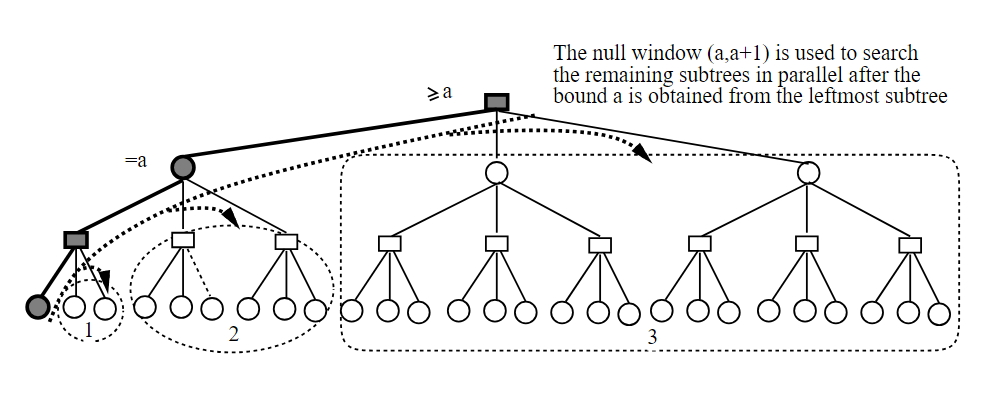
\includegraphics[width=0.8\textwidth]{Imagenes/Bitmap/pvsplitting.png}
    \caption{Principal variation splitting.~\cite{PVSplitting}}
    \label{fig:pv-splitting}
\end{figure}

\begin{lstlisting}[breaklines=true, frame=single]
template<SearchType searchType>
static int alpha_beta_search(std::atomic<bool>& stop, int depth, int ply, int alpha, int beta, SearchContext& context, Board board)
{
    // ...
    // Check if it is in transposition table
    // If it is, return previously calculated evaluation

    generate_legal_moves<ALL_MOVES>(moves, board, &isCheck);
    // ...
    order_moves(moves, board, ply);
    // ...
    
    constexpr SearchType nextSearchType = MAXIMIZING_WHITE ? MINIMIZE_BLACK : MAXIMIZE_WHITE;

    // Search the first move sequentially
    board.make_move(moves[0]);
    int eval = alpha_beta_search<nextSearchType>(stop, depth - 1, ply + 1, alpha, beta, context, board);
    board.unmake_move(moves[0], game_state);
    // ...

    // Alpha-Beta pruning with first move
    if (/*prunned*/) goto end_search;

    // Search remaining moves in parallel
    thread = std::thread([&]() {
        for (int i = 1; i < moves.size(); i++) {
            // ...
            // Alpha-Beta pruning with the remaining moves
            if (/*prunned*/) break;
        }
    });
    
    if (thread.joinable()) {
        thread.join();
    }

end_search:
    // Store entry in tranposition table

    return final_node_evaluation;
}
\end{lstlisting}

\subsubsection{Analysis}

To evaluate the improvement in the new evaluation, we conducted the same 100 game match vs the basic bot version. 

\begin{center}
    \begin{figure}[H]
        \centering
        \ResultBar{15cm}{0.5cm}{32}{5}{63}
        \caption{Multithread Search bot vs basic bot}
        \label{fig:results_multithread_search_bot}
    \end{figure}
\medskip
\end{center}

\noindent The results are slightly worse compared to the match using the material-only evaluation, with 8 more losses than before. This may be due to the increased computational cost of evaluating these additional parameters. Furthermore, although these are abstract concepts commonly used by humans to assess positions, the engine may struggle to find a clear correlation between them and actual positional strength.

\subsection{Late Move Reductions}

We experiment with the use of late move pruning, under the assumption that if our move ordering is good, the best move in the position should be among the first explored moves. We reduce the depth by one unit starting from the tenth movement.

\subsubsection{Analysis}

To evaluate the improvement in the new evaluation, we conducted the same 100 game match vs the basic bot version.

\begin{center}
    \begin{figure}[H]
        \centering
        \ResultBar{15cm}{0.5cm}{48}{15}{37}
        \caption{Reductions Search bot vs basic bot}
        \label{fig:results_reductions_search_bot}
    \end{figure}
\medskip
\end{center}

\noindent The results are worse, with 15 more losses than the version without this aggresive pruning.~\ref{fig:results_pext_move_generator_bot} This could be because our move ordering is not that strong, and the best move in the position sometimes is in the last positions.

\section{Additional tools and work}
\label{sec:tools}

As it was mentioned in Section~\ref{sec:how}, some additional work apart from the engine implementation was done to ensure quality of the final product. This section includes some important specifications and features for the interactive board visualizer and testing worflow.

\subsection{Interactive board visualizer using CustomTkinter}

The board is implemented as a grid of squares, with each square capable of displaying a piece image. Piece images are loaded dynamically from the \texttt{assets} directory, which contains PNG files for each piece.

\vspace{1em}

\noindent The visualizer employs an event-driven architecture, where user actions, such as clicks, trigger events handled by the \texttt{EventManager} class. When the Python script is executed, it ensures that an instance of the engine in release version executable exists, starts a new subprocess with the engine, and launches a window displaying the chessboard and interface.

\begin{figure}[H]
    \centering
    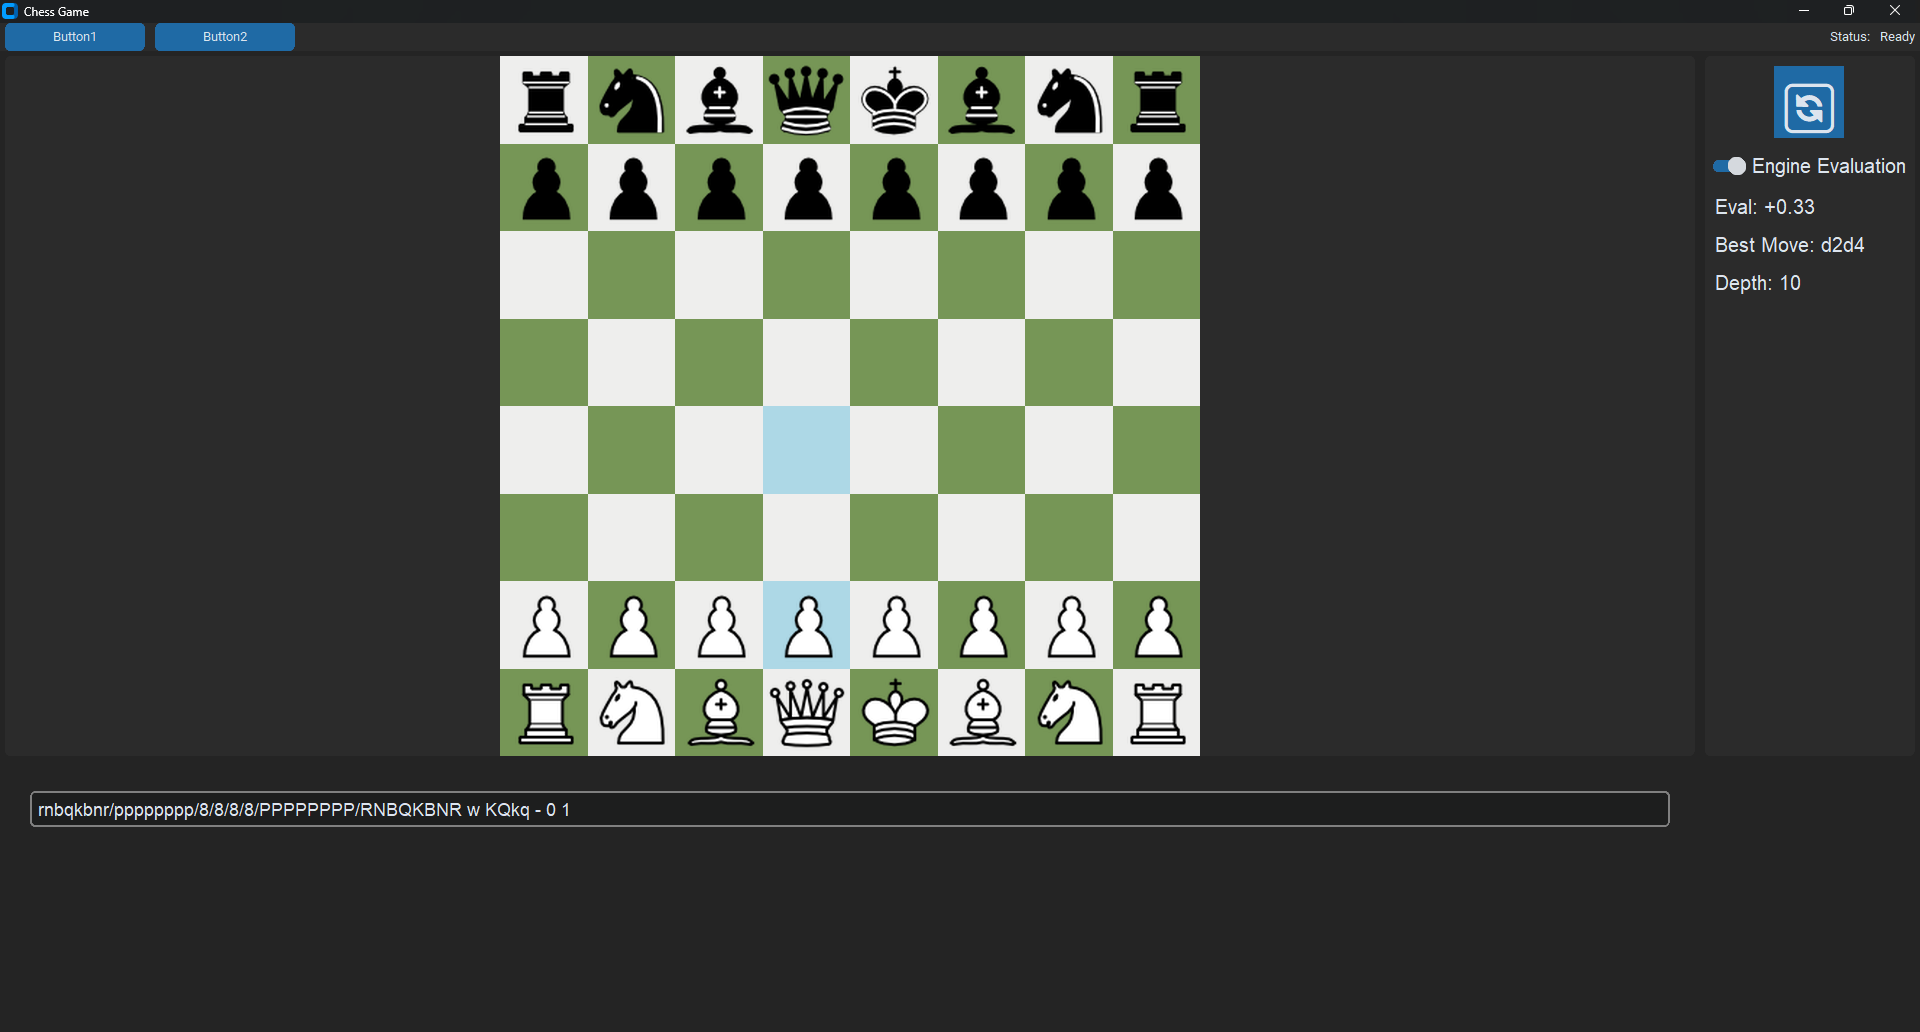
\includegraphics[width=\textwidth]{Imagenes/gui.png}
    \caption{AlphaDeepChess GUI}
    \label{fig:gui}
\end{figure}

On the right panel, there is a switch button to activate and deactivate the evaluation and suggested move in an specific depth. Also, current position's fen on the bottom panel can be modified by exchanging it to a new one.

\subsection{Testing engine strength with Cutechess, Stockfish, and GitHub Actions}

Cutechess and Stockfish can be downloaded from their respective webpages. Then, a JSON file must be provided to Cutechess to configure the available engines. An example of this \texttt{engines.json} file could be:

\vspace{1em}

\begin{lstlisting}[breaklines=true, frame=single]
[
    {
        "name": "AlphaDeepChess",
        "command": "../build/release/AlphaDeepChess",
        "protocol": "uci",
        "options": {}
    },
    {
        "name": "Stockfish",
        "command": "./stockfish/stockfish/stockfish-windows-x86-64",
        "protocol": "uci",
        "options": {
            "UCI_LimitStrength": "true",
            "UCI_Elo": "1500"
        }
    }
]
\end{lstlisting}

\noindent By simply calling the Cutechess CLI with the names of the engines and additional specifications such as search time (\texttt{--st}), the number of games (\texttt{--games}), or depth (\texttt{--depth}), the matches can be executed.

\vspace{1em}

\noindent Finally, automating this process of selecting the versions of the engine and Stockfish we created a workflow using a YAML file.

\vspace{1em}

\noindent This workflow is triggered manually. It includes the following steps:

\begin{itemize}
    \item Setup environment: Install dependencies such as Python packages, Cutechess and Stockfish.
    \item Build the engine: Compile the chess engine from source code.
    \item Run tests: Execute previously designed tests to validate the functionality of the engine using Cutechess CLI.
    \item Export generated data from Cutechess for later analysis.
\end{itemize}

This generated data are the results of the run games that includes:

\begin{itemize}
    \item A \texttt{results.epd} with all the final positions in FEN format.
    \item A \texttt{results.log} with Cutechess additional detailed information like the beginning and end of a game, the summary of the game, and ELO stadistics.
    \item A \texttt{results.pgn} with all the played moves and games.
\end{itemize}
